\documentclass[12pt,a4paper]{report}

\usepackage[backend=biber, style=ieee]{biblatex}
\addbibresource{literature.bib}

\usepackage[utf8]{inputenc}
\usepackage[T1]{fontenc}
\usepackage[ngerman]{babel}
\usepackage{lmodern}
\usepackage{enumitem}
\usepackage{graphicx}

\usepackage{xcolor}
\newcommand{\todo}[1]{\colorbox{red}{\textbf{TODO: #1}}\\}
\newcommand{\question}[1]{\colorbox{yellow}{\textbf{QUESTION: #1}}\\}
\newcommand{\xeno}[1]{\colorbox{pink}{\textbf{TODO XENO: #1}}\\}
\newcommand{\gideon}[1]{\colorbox{green}{\textbf{TODO GIDEON: #1}}\\}

\begin{document}

\begin{titlepage}
  \centering
  {\huge \textbf{Yappi - Developer Happiness} \par}
  {\large IP5 Project \par}
  \vspace{0.5cm}
  {Windisch, August 2025 \par}
  \vspace{0.5cm}

  \begin{tabular}{@{}ll@{}}
    \textbf{Studenten:}    & Xeno Isenegger, Gideon Monterosa \\
    \textbf{Fachbetreuer:} & Norbert Seyff, Nitish Patkar
  \end{tabular}

  \vfill
  {Fachhochschule Nordwestschweiz, Hochschule für Informatik \par}
\end{titlepage}

\chapter*{Abstract}
\newpage

\tableofcontents
\newpage

\listoffigures
\newpage

\listoftables
\newpage

\chapter{Einleitung}

\section{Motivation}
\question{Müssen wir gendern? Entwicklerinnen und Entwickler}

Die Zufriedenheit von Entwicklerinnen und Entwicklern wird, wenn überhaupt, meist nur anhand der
Menge ihrer geleisteten Arbeit gemessen. Dabei entstehen zwangsläufig Defizite, und ein halbjährli-
ches Mitarbeitergespräch erweist sich oft als wenig wirksame Massnahme zur Problemlösung.

Dieses Projekt baut auf einer bestehenden Arbeit auf, in der eine Plattform zur Erfassung der Ent-
wicklerzufriedenheit entwickelt wurde. Die Webapplikation Yappi ermöglicht es Entwicklerinnen und
Entwicklern, ihre Zufriedenheit mit ihrer Arbeit und ihrer aktuellen Situation fortlaufend zu bewerten.
Yappi erfasst emotionale Faktoren wie Happiness sowie weitere Zufriedenheitsindikatoren. Zusätz-
lich können spezifische Aufgaben und Arbeitstypen individuell bewertet werden. Die erhobenen Da-
ten werden anonym auf Teamebene analysiert, um ein fundiertes Verständnis für die Stimmung in-
nerhalb der Teams zu gewinnen.

Entwicklerinnen und Entwickler haben die Möglichkeit, ihre Zufriedenheit für verschiedene Teams zu
erfassen, wodurch gezielte Analysen ermöglicht werden. Unternehmen erhalten dadurch wertvolle
Einblicke, um das Arbeitsumfeld gezielt zu verbessern.

Unser Projekt baut auf Yappi auf und zielt darauf ab, die Erfassung der Zufriedenheit weiter zu opti-
mieren. Es wird untersucht, wie die Daten noch präziser erfasst und ausgewertet werden können,
um langfristige Verbesserungen zu unterstützen. Diese Arbeit dient als Grundlage für ein weiterfüh-
rendes Forschungsprojekt, das sich vertieft mit der Entwicklerzufriedenheit auseinandersetzt und
zusätzliche Erkenntnisse gewinnen soll.

\section{Ziele und Vision}

Yappi wird zu einer umfassenden Plattform weiterentwickelt, die nicht nur die Zufriedenheit misst,
sondern sich nahtlos in den Arbeitsalltag integriert und wertvolle Handlungsempfehlungen liefert.
Dazu werden folgende Kernaspekte umgesetzt:

\subsubsection{Produktivitätsfaktoren identifizieren}

Durch eine tiefere Analyse von Zufriedenheitsindikatoren sollen zentrale Faktoren ermittelt werden,
die sich positiv oder negativ auf die Produktivität und das Wohlbefinden von Entwicklerinnen und
Entwicklern auswirken. Diese Erkenntnisse werden genutzt, um Vorschläge zu Verbesserungsmass-
nahmen abzuleiten.

\subsubsection{Integration in den Arbeitsprozess}

Yappi soll sich direkt in bestehende Arbeitsabläufe einfügen, um die Erfassung der Zufriedenheit
möglichst intuitiv und effizient zu gestalten. Dies kann durch verschiedene Schnittstellen und Erwei-
terungen erfolgen, die eine nahtlose Interaktion ermöglichen.

\subsubsection{Erweiterung um kontextbezogene Daten}

Um ein umfassenderes Bild der Arbeitszufriedenheit zu erhalten, können weitere Einflussfaktoren
berücksichtigt werden. Dazu gehören beispielsweise arbeitsbezogene Rahmenbedingungen oder
individuelle Gesundheits- und Belastungsindikatoren. Diese Daten sollen helfen, ein besseres Ver-
ständnis für langfristige Trends und Zusammenhänge zu entwickeln.

\subsubsection{Intelligente Analyse und Handlungsempfehlungen}

Durch die Integration von AI schnittstellen können gezielte Analysen erstellt und individualisierte
Empfehlungen abgeleitet werden. Dies kann sowohl auf individueller als auch auf Teamebene erfol-
gen, um nachhaltige Verbesserungen im Arbeitsumfeld zu fördern.

\subsubsection{Fazit}

Mit diesen Erweiterungen wird Yappi zu einem essenziellen Bestandteil des Entwickleralltags. Es
bietet nicht nur eine präzisere Erfassung der Zufriedenheit, sondern liefert auch wertvolle Einblicke
und Handlungsempfehlungen, um die Arbeitsbedingungen nachhaltig zu verbessern. Unternehmen
erhalten fundierte Analysen und können gezielt Massnahmen ergreifen, um eine motivierte und pro-
duktive Entwicklergemeinschaft zu fördern.

\section{Fragestellungen}

\begin{enumerate}[label=\Alph*.]
  \item Durch welche Technologien und Schnittstellen kann Yappi erweitert werden,
        um ein reibungsloses und einfaches Erfassen von Zufriedenheitsdaten zu ermöglichen?
        \begin{enumerate}[label=\alph*.]
          \item Entwicklung von Entwickler-Tool-Plugins, die nahtlos in bestehende Arbeitsumgebungen
                integriert werden können, um die Nutzung von Yappi angenehmer und effizienter zu gestalten.
                Diese Plugins sollen Entwicklern ermöglichen, direkt in ihrer bevorzugten Umgebung Feedback
                zu erfassen, ohne den Arbeitsfluss zu unterbrechen. Integration von Yappi in verschiedene
                Plattformen und Tools wie Webbrowser, IntelliJ, Microsoft Teams und Outlook.
        \end{enumerate}
  \item Wie können Gesundheitsdaten in die Auswertung der Entwicklerzufriedenheit einfliessen?
        \begin{enumerate}[label=\alph*.]
          \item Direkte Anbindung der Gesundheitsdaten-API, um relevante Gesundheitsmetriken wie
                Herzfrequenz, Schlafqualität oder Stresslevel automatisch in die Analyse der
                Entwicklerzufriedenheit zu integrieren. Dies ermöglicht eine genauere Einschätzung des
                Wohlbefindens und potenzieller Belastungsfaktoren.
        \end{enumerate}
  \item Wie kann Yappi Teams und Entwickler dabei unterstützen, aus den erfassten
        Zufriedenheitsdaten Handlungsempfehlungen abzuleiten, um die Zufriedenheit und Produktivität
        von Entwicklern zu erhöhen?
        \begin{enumerate}[label=\alph*.]
          \item Entwicklung eines Yappi Coach, der anhand einer detaillierten Analyse der erfassten
                Daten gezielte Tipps zur Verbesserung der Arbeitsweise gibt. Beispielsweise könnte der Coach
                darauf hinweisen, dass Meetings nicht länger als 1,5 Stunden dauern sollten, da längere
                Sitzungen die Zufriedenheit und Konzentration der Entwickler negativ beeinflussen können.
          \item Integration von KI-gestützten Diensten, die auf Basis der gesammelten Gesundheitsdaten
                sowie Zufriedenheits- und Produktivitätsmetriken individuelle Massnahmen vorschlagen. Diese
                KI-gestützten Empfehlungen können Teams dabei helfen, gezielt Optimierungen vorzunehmen, um
                die Arbeitsbedingungen und die Effizienz der Entwickler nachhaltig zu verbessern.
        \end{enumerate}
\end{enumerate}

\chapter{Hintergrund}

\todo{kurze Einleitung}

\section{Ausgangslage}

Yappi ist eine Webplattform zur Erfassung der Entwicklerzufriedenheit und produktionsnaher Kennzahlen. Ziel ist eine regelmässige,
datenbasierte Diskussion im Team und ein besseres Verständnis wiederkehrender Muster der Teamstimmung. Die Vorgängerarbeit
definiert dafür eine klare Produktvision und liefert ein erstes Minimum Viable Product (MVP) als Grundlage. Die Plattform 
fokussiert sich auf Selbst-Reporting zur Auswertung der Entwicklerzufriedenheit. Der Ansatz adressiert typische Schmerzpunkte
agiler Teams und stützt sich auf Interviews, Literatur und abgeleitete Produktziele. Yappi erlaubt die Erfassung von
Happiness-Daten, deren Auswertung im Dashboard und Vergleiche innerhalb eines Teams. Die Lösung ist so ausgelegt, dass in
Retrospektiven datenbasierte Gespräche geführt werden können.

Yappi ist als Open-Source-Projekt veröffentlicht. Die Repositories für Backend, Frontend und Infrastruktur sind getrennt 
organisiert. Eine lauffähige Instanz steht zu beginn dieses Projektes nicht zur verfügung. Die Zielgruppe ist klar beschrieben. 
Angesprochen sind agile Software-Teams, Scrum Master und Product Owner unterschiedlicher Unternehmensgrössen. Die Vorgängerarbeit
hat die methodische Basis gelegt. Sie umfasst Literaturrecherche, Interviews, abgeleitete Problemfelder, User Flows, Produktziele
und die Validierung der Konzeptlösung. Das vorliegende Projekt baut auf dieser Struktur auf und fokussiert nun auf Integration,
Erweiterbarkeit und vertiefte Analytik.

\section{Aktueller technischer Stand}

\begin{description}
  \item[Backend] Das Backend ist mit Spring Boot umgesetzt. Als Datenbank ist PostgreSQL im Einsatz. Die Kommunikation zum Frontend
    erfolgt über REST-Schnttstellen, welche nach dem OpenAPI standart dokumentiert sind.
  \item[Frontend] Das Frontend basiert auf React und Next.js mit TypeScript. Für Aufrufe werden SWR-Hooks verwendet, dabei handelt
    es sich ume eine React library um Daten zu laden. Komponenten werden mit der Library wird shadcn/ui aufgebaut. Die 
    Visualisierungen entstehen mit Recharts. Um die Codequalität sicherzustellen wird ESLint zur statischen Code analyse und 
    Prettier zur automatischen Formatierung nach vordefinierten Guidelines verwendet.
  \item[Authentisierung und Autorisierung] Die Anmeldung erfolgt über OAuth 2.0. Dabei werden Anbieter wie Google oder GitHub 
    über Auth.js unterstützt. Passwörter werden nicht gepseichert. Die Anfragen ans Backend werden mit JSON Web Tokens (JWT) 
    abgesichert.
  \item[Datenmodell] Das relationale Schema umfasst unter anderem Benutzer, Teams, Sprints sowie Umfragetypen für Happiness,
    Emotionen und Work-Kinds.
  \item[Deployment] Die Komponenten sind grösstenteils containerisiert mit Docker. Eine funktionierende CI/CD-Pipeline ist aktuell
    nicht vorhanden. Bestehende Images sind im GitHub Container Registry abgelegt. Für den Betrieb wird eine Linux-VM wie z.B. auf
    der Switch-Engine-Infrastruktur benötigt.
\end{description}
\section{Parallele Entwicklung auf gemeinsamer Codebasis}

\todo{Zusammenarbeit kurz erklären mit Auswirkungen auf unser Projekt}

\section{Stakeholder}

Das Projekt umfasst die folgenden Stakeholder:

\begin{description}
  \item[Primäre Nutzergruppen] Softwareentwickelnde, Scrum Master und Product Owner in agilen Teams. 
  \item[Organisationen] Unternehmen nutzen Yappi, um Kultur und Zusammenarbeit datenbasiert zu verbessern.
  \item[Akademische Stakeholder] Betreuende Dozierende und das Institut an der FHNW welche das Projekt begleiten.
  \item[Betrieb und Entwicklung] Projektteam dieses Projekts und anderer Projekte die auf Yappi aufbauen.
\end{description}

\chapter{Methoden}
\todo{Kanban erwähen}
\section{Projektmethodik}
\section{Prototypen}
\section{Proof of Concepts}
\todo{Abgrenzung bezüglich Datenschutz}
\todo{arc42 erwähen}

\chapter{State of the Art}
\section{Definition von Entwiklerzufriedenheit}

Entwicklerzufriedenheit wird in der Literatur als Balance zwischen positiven und negativen Erlebnissen bei der
Arbeit definiert. Darunter versteht man eine Sequenz von Erfahrungen, bei der häufige positive Emotionen ein
hohes Glücksgefühl erzeugen und häufige negative Erfahrungen das Gegenteil bewirken \cite{sadowski_happiness_2019}.
Auch Industriequellen fassen Entwicklerzufriedenheit als subjektives Wohlbefinden in Bezug auf Arbeitsinhalte
und -umfeld auf, d.h. als Mass für Zufriedenheit, Freude oder innere Zufriedenheit bei der Arbeit \cite{zenhub_2022_nodate}.
Zufriedene Entwickler empfinden demnach mehr Arbeitsfreude und Inhaltlichkeit in ihrer Rolle, was eng mit
der Arbeitsmotivation und dem Engagement bei der Arbeit verknüpft ist \cite{franca_motivation_2020}.

\question{braucht es hier eine citation oder fussnote für den originalen Begriff von flow}
Eng verwendt mit der Zufriedenheit ist der Begriff \textbf{Flow}. In Anlehnung an Csikszentmihalyis Konzept beschreibt
Flow einen Zustand von völliger Vertiefung und hohen Fokus beim Programmieren. Flow tritt dann auf, wenn die Anforderungen
einer Aufgabe im Gleichgewicht mit dem Fähigkeiten des Entwicklers stehen, wodurch man in einen Zustand von intensiver 
Konzentration gelangt. Zufriedene Entwickler gelangen einfacher in einen anhaltenden Flow-Zustand. Unzufriedenheit
hingegen unterbricht diesen Flow, was zu Frustration führt und Schwierigkeiten führt, nach Unterbrechungen wieder in
eine Aufgabe zurückzufinden. Teilnehmer einer Untersuchung berichten, negative Erlebnisse reissen einen aus dem Flow
Zustand und machen es schwer, die Arbeit wieder aufzunehmen \cite{sadowski_happiness_2019}.

Motivation und Zufriedenheit hängen eng zusammen, sind aber konzeptionell unterscheidbar. Motivierte Entwickler sind
zeigen hohes Engagement und Fokus auf ihre Aufgaben, während Zufriedenheiteher durch allgemeines Wohlbefinden und gute
Laune charakerisiert ist. Faktoren wie Autonomie, Kompetenzerleben und Zugehörigkeitsgefühl steigern die intrinsische 
Motivation von Entwicklern, was sich positiv auf ihre Zufriedenheit auswirkt. Zufriedenheit ist zugleich das Ergebnis und
die Voraussetzung von Motivation, zufriedenere Entwickler weisen in der Regel eine höhere Antriebskraft auf, was wiederum ihre
Arbeitszufriedenheit weiter stärkt \cite{franca_motivation_2020}.

Schliesslich spielt auch das Team- und Organisationsklima eine fundamentale Rolle. Eine offene, unterstützende Kultur steigert
nachweislich die zufriedenheit von Entwicklern. Der DORA Report misst die Leistungsfähigkeit von Softwareentwicklungsteams anhand
von vier Schlüsselkennzahlen: Deployment Frequency, Lead Time for Changes, Change Failure Rate und Time to Resore Service. Der DORA
Report von Google basiert auf umfangreichen Wissenschaftlichen Studien und gilt als Branchenstandart. Der report von 2024 betont,
dass Teams mit stabilem, ermutigendem Umfeld bessere Ergebnisse erzielen \cite{google_dora_2024}. Positive Emotionen und ein 
Zugehörigkeitsgefühl im Team fördern den Gruppenzusammenhalt, was wiederum die Teamleistung von Teammitgliedern verbessert. 
Umgekehrt können Umgekehrt können toxische Kulturen oder ständig wechselnde Prioritäten die Zufriedenheit und Motivation 
untergraben, was sich negativ auf die Leistung auswirkt \cite{sadowski_happiness_2019}.

Somit unterstreichen sowohl akademische als auch industrielle Befunde: Entwicklerzufriedenheit entsteht in einem komplexen
Zusammenspiel aus individuellen Faktoren (Flow, Motivation, ...) und Umfeldfaktoren (Team- und Organisationsklima, Arbeitskultur, 
...).

\section{Stand der Forschung und verwandte Arbeiten}

\question{Definitionen für Erfolgsparameter einfügen?}
In den letzen Jahren haben zahlreiche Studien den Zusammenhang zwischen der Entwicklerzufriedenheit und Erfogsparametern wie 
Produktivität, Codequalität und Mitarbeiterbindung untersucht. Bei einer grossangelegten Studie wurden 317 Softwareentwickler
befragt und dabei 42 Konsequenten von Unzufriedenheit sowie 32 Konsequenzen von Zufriedenheit beim Programmieren identifiziert.
Die Ergebnisse Zeigen, dass Entwicklerzufriedenheit messbare Auswirkungen auf den Enwicklungsprozess, die erzeugten 
Software-Artefakte und das Wohlbefinden der Person hat. So führt Unzufriedenheit zu einer Reihe negativer Effekte: verzögerte
Prozessabläufe, nachlässige Arbeitsweise und häufige unterbrechungen des Flows wurden als typische Folgen von negativer Stimmung
genannt. Unzufriedene Entwickler berichten von langen langen Verzögerungen oder Qualitätsproblemen, weil Frustration sie aus dem
Konzept brachte. Zufriedenheit hingegen wirkt sich positiv aus: Zufriedene Entwickler zeigen bessere Problemlösungsfähigkeiten,
höhere Konzentration, berichten von einem anhaltenden Flow Zustand und lernen schneller. Die Ergebnisse legen nahe, dass 
Zufriedenheit die Codequalität begünstigt. Zufriedene Entwickler treffen sorgfältigere langfristige Entscheidungen. Ein Teilnehmer
beschrieb, er dokumentiert seinen Code gründlicher und achten stärker auf Wartbarkeit, wenn er Zufrieden ist 
\cite{graziotin_what_2018}.

Neben akademischen Studien liefern auch Industireumfragen und Community-Studien wertvolle Einblicke. Der jährliche Stack Overflow
Developer Survey etwa spiegelt wieder, dass weiterhin Verbesserungsbedarf besteht. laut der Umfrage 2024 bezeichen sich nur rund 
20\% der Entwickler als wirklich zufrieden in ihrem Job, während etwa 80\% unzufrieden oder "gelassen" (complacent) sind. Diese Zahl
unterstreicht, dass ein grosser Teil der Entwicklergemeinschaft nicht glücklich im Arbeitsumfeld ist. Als Hauptgründe werden oft
Faktoren wie schlechte Work-Life-Balance, zu viele Meetings oder fehlende Anerkennung genannt \cite{stackoverflow_survey_2025}. Eine
Untersuchung von Zenhub kam zu ähnlichen Ergebnissen: Zwar gaben die meisten befragten Entwickler an, überwiegend zufrieden zu sein,
doch lediglich 31\% fühlten sich äusserst zufrieden in ihrer aktuellen Arbeitssituation \cite{zenhub_2022_nodate}. 

Darüber hinaus tragen Anerkennung und Sinnhaftigkeit der Arbeit entscheidend zur Bindung bei. Wenn Entwicklerinnen und Entwickler
stolz auf die Qualität ihrer Projekte sind und regelmässig Wertschätzung für ihre Arbeit erhalten, steigt sowohl ihre Zufriedenheit
als auch ihre Loyalität gegenüber dem Unternehmen \cite{sadowski_happiness_2019,graziotin_what_2018}. Die empirischen Befunde deuten
somit klar darauf hin, dass Entwicklerzufriedenheit kein rein „weiches“ Thema ist, sondern messbare Auswirkungen auf Produktivität,
Codequalität und Personalbindung hat. Zufriedene Entwickler arbeiten effizienter, treffen sorgfältigere Entscheidungen und bleiben
ihrem Team länger erhalten, während Unzufriedenheit mit erhöhten Kosten für Projekte und Rekrutierung verbunden ist.

\todo{evt. Methoden und Instrumente zur Messung der Entwicklerzufriedenheit}
\todo{evt. Technologische und methodische Ansätze in verwandten Arbeiten}
\todo{Forschungslücken}

\section{Bestehende Lösungen und Wettbewerbsanalyse}

Der Markt bietet bereits verschiedene Tools und Plattformen, die Teilaspekte der Entwicklerzufriedenheit adressieren. Im Folgenden
werden einige repräsentative bestehende Lösungen vorgestellt und hinsichtlich ihres Fokus und ihrer Lücken bewertet:

\begin{description}
  \item[Officevibe:] Ein Software-as-a-Service-Tool, das wöchentliche Pulse-Umfragen an Mitarbeitende verschickt. Ziel ist es,
    Engagement und Stimmung im Unternehmen kontinuierlich zu messen. Officevibe bietet anonyme wöchentliche Kurzbefragungen per
    E-Mail oder Chat an, deren Ergebnisse in übersichtlichen Dashboards für Teamleiter aufbereitet werden. Entwicklerteams erhalten
    dadurch Stimmungs-Trendkurven und allgemeines Mitarbeiterfeedback. Allerdings ist Officevibe eher generisch auf
    Mitarbeiterengagement ausgerichtet und liefert keine speziell auf Entwickler zugeschnittenen Kontextdaten, z.B. werden keine
    technischen Metriken aus der Softwareentwicklung einbezogen \cite{courier_officevibe_2025}.

  \item[TeamMood:] Ein schlankes Stimmungsbarometer für Teams, das täglich eine einfache Mood-Abfrage durchführt. TeamMood sendet
    jedem Teammitglied jeden Tag einen kurzen Prompt (per E-Mail, Slack, microsoft teams etc.), in dem die Person mit einem Klick
    ihre aktuelle Stimmung angibt. Die Antworten werden als anonymer Team-Stimmungsverlauf visualisiert, was es erlaubt, Trends über
    die Zeit zu erkennen. Die Hürde zur Teilnahme ist sehr niedrig (niedrigschwelliges Feedback). Jedoch erfasst TeamMood keine
    technischen Prozessmetriken (wie Code-Commits, Buildzeiten o.ä.) und bietet keine automatisierten Empfehlungen. Das bedeutet,
    dass Entwickler und Manager die Stimmungsverläufe selbst interpretieren und Massnahmen ableiten müssen, ohne direkte
    Handlungsempfehlungen durch das Tool \cite{revelo_teammood_2025}.

  \item[Happimeter:] Hervorgegangen aus einem Forschungsprojekt (u.a. TU Wien und MIT) setzt Happimeter auf Wearable Sensoren, um
    einen persönlichen Happiness-Score zu bestimmen. Entwickler tragen z.B. eine Smartwatch mit der Happimeter-App, die
    kontinuierlich physiologische Daten wie Herzfrequenz, Bewegung oder Schlaf erfasst. Ein Machine-Learning-Modell sagt daraus
    die aktuelle Stimmung bzw. den Stresslevel der Person voraus. Auf diese Weise sollen objektive Gesundheitsmetriken mit dem
    subjektiven Wohlbefinden verknüpft werden. Der Ansatz liefert interessante biometrische Einblicke (z.B. Stressspitzen während
    der Arbeit), jedoch fehlt der direkte Bezug zur eigentlichen Entwicklungsarbeit. Happimeter weiss nichts über Tasks, Code oder
    Arbeitskontext, sodass die sensorbasierten Glücks-Werte ohne diesen Kontext schwer zu interpretieren sind
    \cite{budner_making_2017}.

  \item[Code Climate Velocity:] Code Climate Velocity: Eine Datenplattform, die Entwicklungsmetriken aus Git-Repositories analysiert,
    um die Team-Performance zu bewerten. Velocity konzentriert sich voll auf quantitative Software-Engineering-Kennzahlen. Es misst
    etwa die Durchlaufzeit von Pull Requests, die Commit-Frequenz, die Review-Geschwindigkeit und diverse weitere Metriken der
    Entwicklungspipeline. Auch Industrie-Standards wie die vier DORA-Metriken (Deployment Frequency, Lead Time for Changes, Change
    Failure Rate, Mean Time to Restore Service) sind integriert. Dadurch erhalten Führungskräfte einen detaillierten Blick auf
    Code-Qualität, Liefergeschwindigkeit und Prozess-Effizienz. Allerdings fehlen subjektive Zufriedenheitsdaten vollständig, die
    menschliche Stimmungslage der Entwickler wird nicht erfasst. Etwaige Einflüsse von Motivation oder Frustration auf die
    gemessenen Leistungsindikatoren bleiben somit unsichtbar \cite{infoworld_codeclimate_2023}.

  \item[GitHub Insights:] Als integrierter Teil von GitHub bietet Insights grundlegende Analysen zur Repository-Aktivität. In jedem
    GitHub-Repository steht ein Insights-Dashboard zur Verfügung, das Statistiken zu Commits, Pull-Request-Aktivitäten,
    Issue-Verläufen und Release-Frequenzen visualisiert. Teams können so ihre Entwicklungsaktivität und Geschwindigkeit verfolgen
    (“Wie viele PRs werden pro Woche gemerged? Wie oft wird deployed?” etc.). Diese Metriken sind wertvolle Aktivitätsstatistiken,
    berücksichtigen jedoch keine emotionalen Faktoren. GitHub Insights liefert also Kennzahlen zur Produktivität, blendet aber das
    Stimmungsbild der Entwickler aus. Etwa ob eine Phase hoher Commit-Rate auf Überstunden und Stress zurückzuführen ist, bleibt
    unklar \cite{axify_git_2025}.

  \item[Microsoft Viva Insights:] Viva Insights ist Teil von Microsoft 365 und zielt darauf ab, durch Analyse von Arbeitsmustern die
    Produktivität und das Wohlbefinden von Mitarbeitenden zu verbessern. Die Plattform wertet vor allem Kalender- und
    Kommunikationsdaten aus (z.B. E-Mail- und Teams-Nutzung, Meeting-Häufigkeit). Entwickler erhalten z.B. Hinweise, wenn
    Meeting-Überlast droht, oder Vorschläge, regelmässige Fokuszeiten für ungestörtes Arbeiten einzuplanen. Führungskräfte sehen
    aggregierte Team-Insights, etwa ob viele Überstunden anfallen oder wenig Konzentrationsphasen vorhanden sind. Zwar gibt Viva
    nützliche Empfehlungen (z.B. “Schützen Sie wöchentlich 4 Stunden Fokuszeit” oder “Vermeiden Sie Meetings über 1 Stunde”).
    Allerdings werden Wohlbefinden und Zufriedenheit nur indirekt aus den Verhaltensdaten abgeleitet, eine direkte Erfassung der
    Gefühlslage oder ein Bezug zu konkreten Entwickler-Tätigkeiten (Code, Tickets etc.) fehlt vollständig. Somit bleibt die
    emotionale Dimension in Viva Insights eher implizit und generalisiert \cite{zachminers_introduction_nodate}.
\end{description}

Bestehende Lösungen decken jeweils nur einzelne Aspekte der Entwicklerzufriedenheit ab. Engagement-Tools erfassen Stimmungsdaten,
stellen jedoch keinen Bezug zu technischen oder gesundheitlichen Kontextinformationen her. Engineering-Analytics-Tools analysieren
Leistungskennzahlen, berücksichtigen jedoch die emotionale Dimension nicht. Gesundheits-Tracker wiederum messen physiologische Daten,
ohne diese mit der konkreten Entwicklungsarbeit zu verknüpfen. Eine Plattform, die emotionale Faktoren, technischen Kontext und
physisches Wohlbefinden gemeinsam erfasst und daraus konkrete Handlungsempfehlungen ableitet, ist derzeit nicht verfügbar.

\chapter{Konzeptentwurf}

Die im vorhergehenden Kapitel dargestellte Analyse bestehender Lösungen verdeutlicht, dass es derzeit keine Plattform gibt, welche
emotionale Faktoren, technischen Kontext und physisches Wohlbefinden integriert erfasst und daraus konkrete Handlungsempfehlungen
ableitet. Yappi soll genau diese Lücke schliessen und eine einheitliche, praxisorientierte Lösung bieten. Ziel ist es, die
Entwicklerzufriedenheit umfassend zu erfassen und die gewonnenen Erkenntnisse in konkrete Massnahmen zu überführen. Die geplanten
Kernfunktionen umfassen:

\begin{description}
  \item[Integriertes Erfassen im Arbeitsfluss:] Yappi lässt sich nahtlos in den täglichen Entwicklungsprozess einbetten. Durch 
    Plugins für Entwicklungsumgebungen, Browser-Erweiterungen oder Integrationen in Kollaborationstools können Entwickler ihre
    Zufriedenheit direkt in ihrer Arbeitsumgebung erfassen, ohne den Kontext zu wechseln. Dies erhöht die Teilnahmebereitschaft
    und stellt sicher, dass Feedback leicht und unmittelbar gegeben werden kann ohne den Arbeitsfluss zu unterbrechen.
  \item[Automatischer Kontext durch Prozessdaten:] Neben manuellen Stimmungsangaben bezieht Yappi automatisch Kontextinformationen
    aus dem Arbeitsprozess ein. Beispielsweise können Commit-Daten aus Git und Kalendereinträge herangezogen werden, um die Stimmung
    in Bezug zu objektiven Ereignissen zu setzen. So liesse sich erkennen, ob z.B. eine Häufung negativer Stimmungswerte mit vielen
    Meetings korreliert.
  \item[Erweiterung um Gesundheitsmetriken:] Um ein umfassenderes Bild des Wohlbefindens zu erhalten, soll Yappi optional auch
    Gesundheitsdaten einbeziehen. Dies kann durch die Anbindung an gängige Gesundheits-APIs oder Wearables (ähnlich Happimeter)
    erfolgen. Die so gewonnenen zusätzlichen Datenpunkte ermöglichen es, langfristige Entwicklungen zu erkennen und diese im
    Zusammenhang mit Prozess- sowie Zufriedenheitsdaten zu analysieren.
  \item[KI-gestützter Coach mit Handlungsempfehlungen:] Über die reine Datenerfassung hinaus soll Yappi einen intelligenten
    Empfehlungsdienst bereitstellen. Dieser Yappi-Coach analysiert die erfassten Zufriedenheitsdaten, Produktivitätskennzahlen und
    gegebenenfalls Gesundheitsdaten mittels KI-gestützter Verfahren. Auf dieser Grundlage werden gezielte, evidenzbasierte
    Empfehlungen für einzelne Entwicklerinnen und Entwickler sowie für Teams generiert. Beispielsweise könnte der Coach vorschlagen,
    die Dauer von Team-Meetings auf höchstens 1,5 Stunden zu begrenzen, wenn längere Sitzungen mit sinkender Zufriedenheit
    einhergehen. Ebenso kann er empfehlen, nach vier Stunden konzentrierter Entwicklungsarbeit eine Pause einzulegen, sofern die
    Analyse zeigt, dass dies die Zufriedenheit steigert. Ziel ist es, konkrete Handlungsimpulse zu geben, die sowohl das
    individuelle Wohlbefinden als auch die Teamproduktivität verbessern.
\end{description}

Durch die Kombination dieser Aspekte entsteht mit Yappi eine zentrale Plattform, die kontinuierliches Stimmungs-Tracking,
automatisierte Kontextdaten aus dem Arbeitsprozess, Gesundheitsmetriken und KI-gestützte Handlungsempfehlungen integriert. Ziel ist
es, die Entwicklerzufriedenheit nicht nur präzise zu erfassen, sondern die gewonnenen Erkenntnisse unmittelbar in nachhaltige
Verbesserungen des Arbeitsalltags zu überführen. Unternehmen erhalten damit eine fundierte Entscheidungsgrundlage, um gezielt
Massnahmen zur Förderung einer motivierten, gesunden und leistungsfähigen Entwicklergemeinschaft umzusetzen. Die nachfolgenden
Abschnitte greifen diese Kernaspekte auf und verknüpfen sie mit weiteren Konzeptbestandteilen, um ein ganzheitliches Lösungsdesign
zu entwickeln.

\section{Yappi als Integrationsplattform}

Die Erweiterung von Yappi zu einer Integrationsplattform ist notwendig, um Daten aus unterschiedlichen Quellen sicher und 
zuverlässig zu erfassen. Neben Prozessdaten wie Commits oder Meeting-Aktivitäten sollen auch Gesundheitsdaten aus externen
Companion Apps einbezogen werden. Dies erfordert eine Architektur, welche den Datenaustausch zwischen Yappi und externen Anwendungen
standardisiert und absichert. Zentrales Element ist ein API-Key-basiertes Authentifizierungsverfahren, das autorisierte Anwendungen
eindeutig identifiziert und deren Zugriff kontrolliert. Auf dieser Basis können Daten aus heterogenen Quellen in ein einheitliches
System integriert werden.

\subsubsection{Kommunikationsmechanismus}

Für die Kommunikation zwischen Companion-Anwendungen und dem Yappi Backend wurde bewusst auf einen API-Key-basierten Mechanismus
gesetzt, anstatt die bestehende JWT-basierte Authentifizierung des Frontends zu verwenden. JWTs eignen sich vor allem für die
Authentifizierung einzelner Nutzer in interaktiven Sitzungen. Sie erfordern in der Regel eine vorgelagerte Benutzeranmeldung und
regelmässige Token-Erneuerung. Dieser Ablauf ist für Companion-Anwendungen, die im Hintergrund oder automatisiert Daten erfassen
und übertragen, nicht optimal. Diese würden durch die Notwendigkeit einer manuellen Anmeldung in ihrer Funktionalität eingeschränkt.

Der API-Key-Mechanismus wurde entwickelt, um diesen Anforderungen gerecht zu werden. Jeder Nutzer verfügt über einen persönlichen
API-Key, der in der Webanwendung einmalig generiert wird. Dieser Schlüssel wird manuell in den gewünschten Companion-Anwendungen
hinterlegt. Bei jeder Anfrage an das Backend wird der API-Key im HTTP-Header übermittelt. Das Backend prüft die Gültigkeit des 
Schlüssels und ordnet die Anfrage dem entsprechenden Nutzerkonto zu. So wird sichergestellt, dass nur autorisierte Clients im
Namen des Nutzers Daten übermitteln können. API-Keys lassen sich bei Bedarf widerrufen oder rotieren. Durch diesen Mechanismus
können Companion-Anwendungen zuverlässig und ohne Benutzerinteraktion mit Yappi kommunizieren, während gleichzeitig ein hohes Mass
an Sicherheit gewährleistet ist.

Durch diesen Mechanismus können Companion-Anwendungen zuverlässig und ohne wiederkehrende Benutzerinteraktion mit Yappi 
kommunizieren, während gleichzeitig ein hohes Mass an Sicherheit gewährleistet ist.

\subsubsection{Systemarchitektur der Integrationsplattform}

\begin{figure}[!htbp]
  \centering
  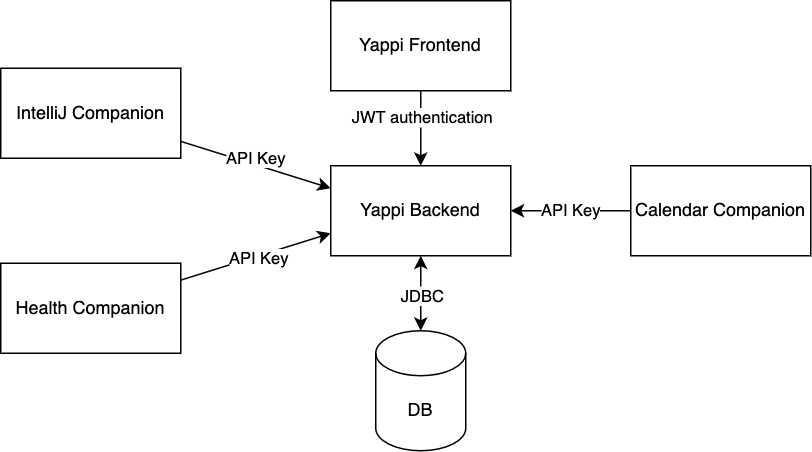
\includegraphics[width=0.95\textwidth]{../figures/plattform-system-diagram.drawio.png}
  \caption{Systemarchitektur der Yappi-Integrationsplattform}
  \label{fig:systemarchitektur}
\end{figure}

Das in Abbildung \ref{fig:systemarchitektur} dargestellte Architekturdiagramm zeigt die zentralen Komponenten der 
Yappi-Integrationsplattform sowie deren Anbindung an externe Companion-Anwendungen. Im Zentrum befindet sich das Yappi Backend,
das als zentrale Schnittstelle für alle eingehenden Daten und Anfragen fungiert.

Das Yappi Frontend verwendet die bestehende JWT-basierte Authentifizierung zur Verwaltung von Nutzersitzungen. Externe
Companion-Apps, wie beispielsweise die IntelliJ-, Health- oder Calendar-Companion, sind über einen API-Key-Mechanismus angebunden.
Dieser gewährleistet, dass nur registrierte und autorisierte Clients Daten an das System übermitteln können. Alle eingehenden
Daten werden vom Backend in der dargestellten Datenbank (DB) persistiert.

\subsubsection{Sicherheit}

Der API-Key-Mechanismus der Integrationsplattform ist so konzipiert, dass er eine sichere und kontrollierte Anbindung externer
Companion-Anwendungen ermöglicht. Jeder API-Key ist eindeutig einem Nutzerkonto zugeordnet und wird in der Webanwendung einmalig
generiert. Die Generierung erfolgt über eine abgesicherte Benutzeroberfläche, wodurch sichergestellt ist, dass ausschliesslich
berechtigte Nutzer einen Schlüssel anlegen können. Zur Übertragungssicherheit wird der API-Key ausschliesslich über verschlüsselte
Verbindungen (HTTPS) zwischen der Companion-Anwendung und dem Backend übertragen.

Im Backend erfolgt eine serverseitige Validierung, bei der der Schlüssel auf Gültigkeit und Zuordnung geprüft wird. Die Schlüssel
werden dabei nicht im Klartext gespeichert, sondern in sicherer Form (z. B. gehasht) abgelegt, um auch bei einem möglichen
Datenbankzugriff unbefugten Gebrauch zu verhindern. Ein kompromittierter API-Key kann jederzeit durch den Nutzer oder einen
Administrator gesperrt oder durch einen neuen ersetzt werden.

\subsubsection{Ablauf der API-Key Erstellung und -Verwendung}

Abbildung \ref{fig:apikey-swimlane} zeigt den Ablauf der Erstellung und Verwendung des API-Keys innerhalb der
Yappi-Integrationsplattform. Die Darstellung erfolgt als Swimlane-Diagramm und verdeutlicht die beteiligten Akteure sowie deren
Interaktionen während des gesamten Prozesses.

\begin{figure}[!htbp]
  \centering
  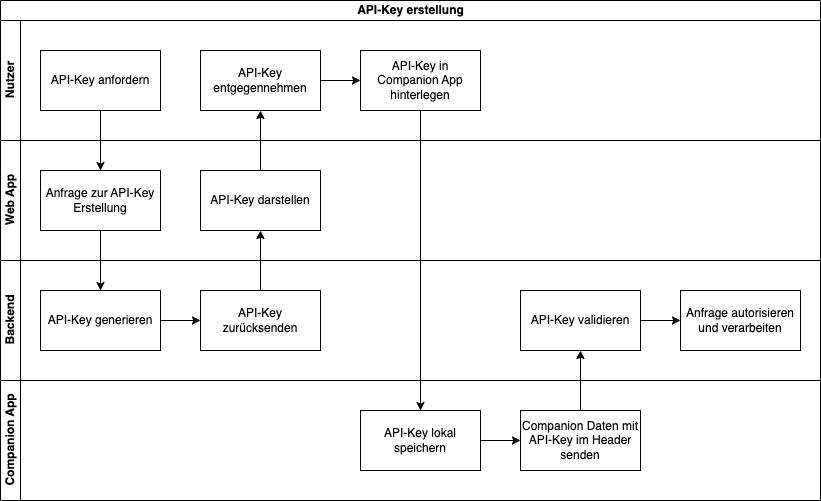
\includegraphics[width=0.95\textwidth]{../figures/apikey-swimlane-diagram.drawio.png}
  \caption{Ablauf der API-Key Erstellung und -Verwendung in Yappi}
  \label{fig:apikey-swimlane}
\end{figure}

Der Prozess beginnt mit der einmaligen Generierung des API-Keys durch den Nutzer in der Webanwendung. Nach der Erstellung wird der
Schlüssel in der Companion-App hinterlegt und dort dauerhaft gespeichert. Jede Datenanfrage der Companion-App an das Backend
enthält den API-Key im HTTP-Header, woraufhin das Backend den Schlüssel validiert und die Anfrage bei positiver Prüfung
autorisiert. Dieser Ablauf stellt sicher, dass ausschliesslich autorisierte Anwendungen im Namen eines Nutzers Daten an Yappi
übermitteln können.

\section{Companion Apps}
\todo{kurze Einleitung}

\subsection{Integration in die Entwicklungsumgebung}

\xeno{rework}

Yappi wird direkt in die integrierte Entwicklungsumgebung (IDE) eingebunden, um den Arbeitsfluss von Entwicklerinnen
und Entwicklern nicht zu unterbrechen.Als primäre Zielplattform eignet sich ein Plugin für IntelliJ IDEA,
eine der weltweit am häufigsten genutzten Java-Entwicklungsumgebungen von JetBrains.
Die Wahl von IntelliJ IDEA basiert auf drei Hauptfaktoren: hohe Verbreitung im professionellen Java-Umfeld,
umfangreiche Plugin-Schnittstellen zur Integration externer Funktionen und Unterstützung mehrerer Programmiersprachen
und Build-Systeme, was den Einsatz auch in heterogenen Entwicklungsteams ermöglicht.
Die unmittelbare Einbettung in die gewohnte Arbeitsoberfläche erlaubt die Erfassung von Zufriedenheitsdaten ohne Kontextwechsel.

Die Integration trägt dazu bei, den Flow-Zustand zu erhalten.
Flow bezeichnet einen Zustand tiefer Konzentration, der nur entsteht, wenn Anforderungen und Fähigkeiten
im Gleichgewicht stehen und Unterbrechungen vermieden werden.
Kontextwechsel zu externen Tools oder Browsern können diesen Zustand unterbrechen und damit Produktivität sowie Zufriedenheit verringern.
Das IntelliJ-Plugin reduziert solche Unterbrechungen, indem es Feedbackprozesse unmittelbar in den bestehenden Arbeitskontext integriert.

Eine Post-Commit-Aktion ermöglicht es, direkt nach einem abgeschlossenen Commit ein kurzes Feedback abzugeben.
Dadurch entfällt der Umweg über die Webplattform von Yappi, was die Bedienung beschleunigt und die Gefahr von Befragungsmüdigkeit verringert.
Kurze, kontextbezogene Abfragen im richtigen Moment erhöhen die Teilnahmebereitschaft und verbessern die Datenqualität.

Ziel ist ein Erfassungsprozess, der unauffällig, effizient und vollständig in den Entwicklungsprozess integriert ist.


\subsection{Integration von Kalenderdaten}
\xeno{}
\todo{Sytemdiagramm}

Ein vollständiges erfassen der Entwicklerzufriedenheit erfordert die Berücksichtigung aller Arbeitsaspekte,
insbesondere auch Besprechungen (Meetings). Empirische untersuchungen zeigen, dass Entwickler durchschnittlich zwischen
10,9 Stunden und 16,5 Stunden pro Woche in Besprechungen verbringen. Ein erheblicher Teil dieser Zeit wird insbesondere
bei grossen oder ungünstig terminierten Besprechungen als wenig produktiv bewertet.
Eine hohe Meetingfrequenz kann den Arbeitstag fragmentieren und den Flow unterbrechen \cite{stray_understanding_2020, meyer_today_2021}.

Ziel dieses Konzeptentwurf ist die Entwicklung einer Kalendererweiterung für Yappi, welche durch das Integrieren des Persönlichen Kalender
in die bestehenden Webanwendung Yappi und einer Companion-App welche durch eine Browser-Erweiterung einsicht in die Meetings der Entwickler ermöglicht.
Die Erweiterung soll nach Ende eines Meetings automatisch, den Entwickler nach Feedback abfragen und die Ergebnisse davon in Yappi für weitere Auswertungen bereitstellen.

\subsubsection{Messung der Meetingqualität}
\xeno{quelle einbetten}
Zur Bewertung werden sieben Kriterien definiert. Diese sind in Anlehnung an Best Practices und gängige Meeting-Umfrageinstrumente ausgewählt:

\begin{enumerate}
    \item \textbf{Zielklarheit und Relevanz} \\
    Prüft, ob die Meetingziele klar formuliert und relevant waren. Eine präzise Agenda und eindeutige Zieldefinition steigern die Produktivität.

    \item \textbf{Inhaltliche Tiefe und Verständlichkeit} \\
    Bewertet, ob Themen angemessen tief und zugleich verständlich behandelt wurden. Unnötige Detailfülle ist zu vermeiden.

    \item \textbf{Zeitmanagement} \\
    Umfasst Pünktlichkeit beim Start und Einhaltung der geplanten Dauer. Studien empfehlen, Meetingzeiten bewusst zu verkürzen (z. B. 25 statt 30 Minuten), um Effizienz zu erhöhen.

    \item \textbf{Moderation und Beteiligung} \\
    Erfasst die Qualität der Moderation und die aktive Einbindung der Teilnehmenden. Eine hohe Beteiligungsquote gilt als Indikator für Interaktivität.

    \item \textbf{Ergebnisorientierung} \\
    Misst, ob konkrete Entscheidungen oder Aufgaben resultierten. Die Anzahl abgeschlossener Aktionspunkte kann als Kennzahl dienen.

    \item \textbf{Allgemeine Zufriedenheit} \\
    Ermittelt das subjektive Gesamturteil, beispielsweise auf einer Skala von 1 bis 10.

    \item \textbf{Meetingdauer} \\
    Vergleicht geplante mit tatsächlicher Dauer und bewertet die Angemessenheit.
\end{enumerate}

Diese Kriterien ermöglichen ein umfassendes Bild der Meetingqualität und liefern Ansatzpunkte für Verbesserungen.

\subsubsection{Kalenderintegration auf Basis offener Standards}

Zur automatischen Erkennung relevanter Meetings wird eine Anbindung an das Kalendersysteme des Entwickler vorgesehen.
Wichtig dabei ist es einen Offenen Standard zu verwenden um eine möglichst hohe Kompatibilität mit Kalendersystemen zu schaffen.
Grundlage dazu bildet das weit verbreitete iCalendar-Format (ICS), das von nahezu allen gängigen Plattformen unterstützt wird.
Das Konzept sieht vor, dass der Nutzer in Yappi auf seinem Profil den zugriff auf den Kalender hinterlegen kann.
Regelmässig werden die auf einen vom Nutzer im Kalender erstellten Kalendereinträge in die Datenbank synchronisiert.
Auf dieser Basis kann die Anwendung automatisch identifizieren, wann ein Meeting stattfindet.
Dadurch lassen sich Feedback-Anfragen unmittelbar nach dem Ende einer Besprechung auslösen, ohne dass der Nutzer manuell eingreifen muss.

Die Synchronisation des Kalender erfolgt ausschliesslich lesend, um Eingriffe in persönliche Kalender zu vermeiden.
Alle übermittelten Kalenderinformationen werden vertraulich behandelt und ausschliesslich für den definierten Zweck genutzt.
Informationen zu Kalendereinträge sind nur für den Nutzer persönlich einsehbar.

Durch diese Anbindung entfällt das manuelle Erfassung von Kalendereinträgen. Meetings werden automatisch erkannt,
Änderungen übernommen und die Nutzer benachrichtigt. So entsteht ein nahtloser integrierter feedback flow um die
Zufriedenheitsdaten von Meetings für die Entwickler zu erheben.

\subsubsection{Companion-App als Feedback-Trigger}

Die Companion-App wird als Browsererweiterung umgesetzt, um eine direkte Interaktion mit den Entwicklern zum richtigen
Zeitpunkt zu ermöglichen. Nach dem Ende eines im Kalender erfassten Meetings erhält der Nutzer eine Benachrichtigung,
die zur Abgabe einer kurzen Bewertung auffordert. Diese zeitnahe Erhebung stellt sicher, dass Eindrücke und Wahrnehmungen
noch frisch sind und die Datenqualität hoch bleibt. Die Interaktion erfolgt freiwillig, um Befragungsmüdigkeit zu vermeiden,
und ist so gestaltet, dass die Beantwortung wenige Sekunden benötigt. Durch die Integration in den Browser wird kein
zusätzlicher Systemwechsel nötig, wodurch die Hemmschwelle zur Teilnahme sinkt.

\subsubsection{Datenverarbeitung und Auswertung}

Die erhobenen Feedbackdaten werden ausschliesslich auf dem Yappi-Server verarbeitet.
Vor der Auswertung erfolgt eine Anonymisierung, um Rückschlüsse auf einzelne Personen zu verhindern.
Für jedes Meeting werden aggregierte Kennzahlen, wie Durchschnittswerte der sieben Kriterien oder Verteilungen der Bewertungen, berechnet.
Diese werden nur dann angezeigt, wenn eine vordefinierte Mindestanzahl an Rückmeldungen vorliegt.
Neben der Auswertung einzelner Meetings können über längere Zeiträume Trends analysiert und Optimierungsmassnahmen evaluiert werden.

\subsubsection{Integration in die Yappi Webanwendung}

Die bestehenden Funktionen von Yappi werden um einen Bereich zur Meetinganalyse ergänzt.
Entwickler sehen hier ihre eigenen Feedbackabgaben und offene Anfragen.
Auf der Teamebene kann auf aggregierte, anonymisierte Auswertungen zu den Meetings ihres Teams zugegriffen werden.
Die Konfiguration der Kalenderintegration und der Verbindung zur Companion-App wird im Nutzerprofil zentral verwaltet.
Dadurch bleibt die Erweiterung vollständig in die bestehende Systemarchitektur eingebettet und benötigt keine separaten Plattformen.

\subsection{Integration von Gesundheitsdaten}

Gesundheitsdaten können wertvolle Zusatzinformationen zur Entwicklerzufriedenheit liefern. Sie ergänzen subjektive Stimmungsangaben
um objektive Messwerte, die Rückschlüsse auf Belastung und Erholung ermöglichen. Durch die Anbindung an etablierte Schnittstellen
wie Apple Health Kit oder Garmin Health API lassen sich Metriken wie Schlafqualität, Herzfrequenz oder Stressindikatoren 
automatisiert erfassen. Diese Daten bilden zusammen mit den Prozess- und Zufriedenheitsmetriken eine erweiterte Grundlage, um
Korrelationen zwischen physischem Wohlbefinden und Arbeitszufriedenheit zu erkennen und gezielte Massnahmen abzuleiten.

\subsubsection{Auswahl relevanter Gesundheitsmetriken}

Die Integration von Gesundheitsdaten in Yappi soll das subjektive Stimmungsbild ergänzen und objektive Indikatoren für Belastung,
Erholung und generelles Wohlbefinden liefern. Subjektive Zufriedenheitsangaben geben wertvolle Einblicke in die aktuelle emotionale
Lage. Physiologische Metriken hingegen erfassen Veränderungen, die den Betroffenen nicht immer bewusst sind. Beide Perspektiven zu
kombinieren ermöglicht eine fundiertere Analyse potenzieller Einflussfaktoren auf die Arbeitszufriedenheit von Entwicklerinnen und
Entwicklern.

Für die Auswahl der relevanten Gesundheitsmetriken wurden drei Kriterien herangezogen:

\begin{itemize}
  \item \textbf{Wissenschaftlich belegter Zusammenhang} mit Arbeitszufriedenheit oder Leistungsfähigkeit.
  \item \textbf{Technische Messbarkeit} mittels gängiger Wearables bzw. Smartphone-Sensoren.
  \item \textbf{Integrationsfähigkeit} über etablierte Schnittstellen wie Apple Health Kit oder die Garmin Health API.
\end{itemize}

Basierend darauf wurden folgende vier Metriken ausgewählt:

\begin{enumerate}
  \item \textbf{Schlafdauer}\\
        Schlafdauer ist ein zentraler Prädiktor für kognitive Leistungsfähigkeit, emotionale Regulation und Motivation. Chronisch 
        verkürzter Schlaf führt zu verminderter Aufmerksamkeitsspanne, reduzierter Problemlösefähigkeit und einer erhöhten 
        Anfälligkeit für negative Stimmungslagen. Personen mit ausreichendem, qualitativ hochwertigem Schlaf weisen höhere
        Arbeitszufriedenheit, geringere Reizbarkeit und bessere soziale Interaktionen am Arbeitsplatz auf. Besonders in
        wissensintensiven Tätigkeiten wie der Softwareentwicklung, bei denen hohe Konzentration und Kreativität erforderlich sind,
        kann Schlafmangel die Produktivität stark mindern \cite{opoku_sleep_2023}.

  \item \textbf{Ruheherzfrequenz (RHR)}\\
        Die Ruheherzfrequenz reflektiert den Grundzustand des Herz-Kreislauf-Systems und reagiert empfindlich auf chronische 
        Belastungen wie Stress oder Überarbeitung. Eine dauerhaft erhöhte RHR ist mit  reduzierten Erholungsphasen assoziiert.
        In arbeitspsychologischen Studien wurde ein signifikanter Zusammenhang zwischen hohem Job-Strain, erhöhter RHR und niedrigerer Arbeitszufriedenheit festgestellt. Für Entwicklerinnen und Entwickler kann eine kontinuierliche Überwachung der RHR
        helfen, Phasen erhöhter Belastung zu erkennen, noch bevor subjektive Erschöpfung spürbar wird \cite{eriksson_rhr_2016}.

  \item \textbf{Stress (Herzratenvariabilität, HRV)}\\
        Die Herzratenvariabilität beschreibt die zeitliche Variation zwischen aufeinanderfolgenden Herzschlägen und gilt als
        sensibler Indikator für die Funktionsbalance des autonomen Nervensystems. Eine hohe HRV weist auf ein flexibles, gut
        reguliertes System hin, das Belastungen effizient kompensieren kann. Eine niedrige HRV hingegen signalisiert anhaltenden
        Stress oder unzureichende Erholung. In Kombination mit subjektiven Zufriedenheitsdaten kann die HRV helfen, versteckte
        Stressmuster zu identifizieren, die sonst unentdeckt bleiben würden \cite{borchini_hrv_2012}.

  \item \textbf{Aktivitätsminuten und Schritte}\\
        Körperliche Aktivität wirkt sich positiv auf mentale Gesundheit, Energielevel und Stimmung aus. Schon moderate Bewegung
        reduziert Stress, verbessert die Schlafqualität und steigert die Arbeitszufriedenheit. Diese lässt sich durch die täglichen
        Schritte oder die aktiven Minuten messen. Für sitzende Berufe wie die Softwareentwicklung kann regelmässige Bewegung das
        Risiko von Ermüdung und Motivationsverlust verringern. Mitarbeitende mit höherem Aktivitätsniveau klagen seltener über
        emotionale Erschöpfung und haben eine insgesamt positivere Einstellung zur Arbeit \cite{dallmeyer_activity_2023}.
\end{enumerate}

Diese Metriken ermöglichen eine gezielte Verknüpfung zwischen erholungs- und gesundheitsbezogenen Faktoren sowie den erhobenen
Zufriedenheits- und Prozessdaten. Damit lassen sich Muster identifizieren, die potenzielle Belastungssituationen aufzeigen und 
gezielte Massnahmen zur Förderung von Wohlbefinden, Motivation und Leistungsfähigkeit ermöglichen.

\subsubsection{Quellen und Schnittstellen für Gesundheitsdaten}

Für die Integration von Gesundheitsdaten wurden mehrere Optionen geprüft. Im Mittelpunkt standen die Garmin Health API sowie Apple
Health Kit. Beide Quellen decken relevante Metriken wie Schritte, Herzfrequenz, Schlaf und Stress/HRV ab, unterscheiden sich jedoch
deutlich hinsichtlich Zugangsmodell, Datenschutzmechanismen, Integrationsaufwand und Eignung für nicht-kommerzielle 
Forschungsprojekte.

\begin{description}
  \item[Garmin Health API] Die Garmin Health API stellt über eine REST-Schnittstelle umfangreiche Tages- und Aktivitätsmetriken 
    bereit. Die Daten werden in der Regel nach dem Gerätesync via über die Mobile Applikation von Garmin bereitgestellt und in
    JSON ausgeliefert. die Plattform unterstützt Pull- und Push-Modelle, sodass auch eine ereignisgetriebene Integration möglich
    ist. Der Zugang ist für genehmigte Business-Developer vorgesehen. Für die kommerzielle Nutzung fallen in der Regel
    Lizenzgebühren an. Diese geschäftliche Ausrichtung sowie die erforderliche formale Zulassung machen die direkte Nutzung für
    ein kleines, nicht-kommerzielles Forschungsprojekt unpassend. Zwar existieren Forschungsprogramme und Partnerlösungen rund um
    Garmin, diese sind jedoch üblicherweise an formelle Kooperationen, Vertragsaufwände und teils Kosten gebunden, was die
    Umsetzungshürde erhöht \cite{garmin_healthapi_2025}.
  \item[Apple Health Kit] Health Kit dient auf iOS als zentrales, lokales Datenrepository für Gesundheits- und Fitnessdaten von 
    iPhone, Apple Watch und angebundenen Geräten/Apps. Der Zugriff erfolgt feingranular pro Datentyp und erfordert stets explizite
    Nutzerzustimmung (Lesen/Schreiben getrennt). Daten liegen verschlüsselt auf dem Gerät. Apps erhalten nur Zugriff auf die
    explizit freigegebenen Kategorien. Für die Integration stehen dokumentierte APIs und Query-Muster zur Verfügung. Eine
    serverseitige Drittplattform ist nicht erforderlich, wodurch Architektur, Betrieb und Datenschutzfolgenabschätzung vereinfacht
    werden \cite{apple_healthkit_2025}.
\end{description}

Da die Garmin Health API primär für kommerzielle Anwendungen vorgesehen ist und der beantragte Zugang für dieses Projekt nicht
gewährt wurde, wurde Apple Health Kit als geeignetere Datenquelle ausgewählt. Für die Umsetzung bedeutet dies, dass eine
iOS-Anwendung entwickelt wird, die die relevanten Daten aus Apple HealthKit ausliest und an Yappi überträgt.

\section{Yappi Coach}
\todo{Ausgearbeitets Konzept dokumentieren}
\question{hier erwähnen dass umsetzung erst im nächsten projekt?}

\section{Konzeptevaluation}

Ziel der Evaluation war es, die Relevanz der im Konzeptentwurf beschriebenen Erweiterungen von Yappi aus
Sicht der Hauptnutzer zu überprüfen.
Hierzu wurde eine Umfrage erstellt, die alle vorgesehenen Konzepte und deren Funktionen abdeckte.
Die Bewertung erfolgte mit einer Likert-Skala von 0 bis 10, wobei 0 „sehr unwichtig“ und 10 „sehr wichtig“ bedeutet.
Eine Likert-Skala ist ein in der Sozialforschung weit verbreitetes Verfahren, bei dem Teilnehmende ihre Zustimmung
oder Ablehnung zu einer Aussage stufenweise angeben können.
An der Befragung nahmen acht individuelle Softwareentwickler teil.

\begin{figure}[!htbp]
  \centering
  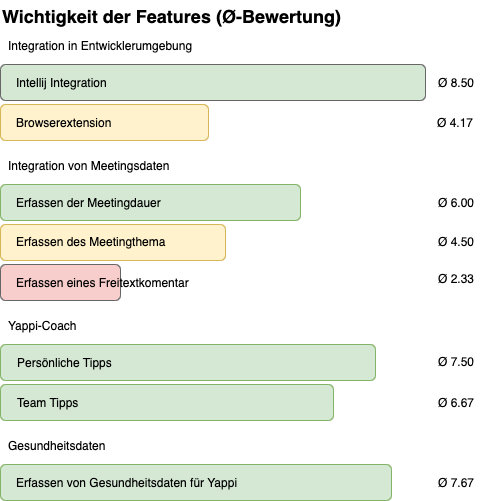
\includegraphics[width=0.85\textwidth]{../figures/konzept-eval-feature-wichtigkeit.drawio.png}
  \caption{Durchschnittsbewertung der Konzeptfunktionen auf einer Likert-Skala von 0 = sehr unwichtig bis 10 = sehr wichtig.}
  \label{fig:konzept-eval-feature-wichtigkeit}
\end{figure}

Die Abbildung~\ref{fig:konzept-eval-feature-wichtigkeit} zeigt die nach Themen gruppierten Durchschnittsbewertungen.
Am höchsten bewertet wurden Funktionen mit direkter Integration in den Arbeitsfluss, wie das IntelliJ-Plugin (8,50)
oder die Erfassung von Gesundheitsdaten (7,67).
Niedrigere Werte erhielten Funktionen, die manuelle Eingaben erfordern, insbesondere Freitextkommentare zu Meetings (2,33).

Die Umfrage diente nicht nur der Bestätigung der Konzeptideen, sondern auch der Priorisierung und Optimierung einzelner Funktionen.
So ergab sich aus den Rückmeldungen, dass die Meetingumfrage als kompakter Frageblock mit Auswahloptionen gestaltet wird,
während Freitextfelder nur ergänzend zum Einsatz kommen.
Damit wird der Aufwand für die Teilnehmenden reduziert und die Wahrscheinlichkeit für regelmässige Rückmeldungen erhöht.

\chapter{Implementierung}
\section{Zugriffskontrolle über API-Keys}

    Das API-Key-System dient der sicheren und eindeutigen Authentifizierung externer Dienste gegenüber der \texttt{Yappi-Companion}-API.
    Anstelle von Benutzeranmeldedaten verwenden Clients einen statisch generierten API-Key, der für den jeweiligen Nutzer erstellt und ausschliesslich diesem zugeordnet ist.
    Dies ermöglicht den kontrollierten Zugriff auf geschützte Endpunkte, ohne dass sensible Login-Daten offengelegt oder dauerhaft gespeichert werden müssen.

    Über einen gültigen API-Key können autorisierte Clients Anfragen an Endpunkte mit dem Pfadpräfix \texttt{/companion/} stellen.
    Beispielsweise kann der Fragenblock mit der ID~\texttt{1} wie folgt abgerufen werden:

    \begin{verbatim}
        GET https://yappi.dev/companion/questionblocks/1
        X-API-KEY: <api-key>
    \end{verbatim}


    \paragraph{Datenbank}
    Die Tabelle \texttt{api\_key} speichert die Metadaten und API-Keys.

    \begin{table}[!htbp]
    \centering
    \begin{tabular}{|l|l|p{9cm}|}
    \hline
    \textbf{Spalte} & \textbf{Datentyp} & \textbf{Beschreibung} \\
    \hline
    \texttt{id} & SERIAL & Primärschlüssel, auto-inkrementierend \\
    \texttt{user\_id} & INTEGER & Fremdschlüssel auf \texttt{users.id} \\
    \texttt{hashed\_key} & TEXT & Gesalteter Hash des API-Keys (z.\,B. BCrypt oder Argon2) \\
    \texttt{created\_at} & TIMESTAMPTZ & Zeitpunkt der Erstellung des Keys \\
    \texttt{expires\_at} & TIMESTAMPTZ & Optionales Ablaufdatum \\
    \texttt{active} & BOOLEAN & Aktivierungs-Flag, um Keys ohne Löschung zu sperren \\
    \hline
    \end{tabular}
    \caption{Schema der Tabelle \texttt{api\_key}}
    \label{tab:api_key_schema}
    \end{table}

    \paragraph{Backend-Komponenten}
    \begin{itemize}
      \item \textbf{Entität} (\texttt{ApiKey.java}) — Abbildung der Tabelle \texttt{api\_key} als JPA-Entität, ohne Feld für den rohen Key.
      \item \textbf{Repository} (\texttt{ApiKeyRepository.java}) — Zugriff auf API-Key-Datensätze, inkl. Suche nach Key-Präfix.
      \item \textbf{Util-Klasse} (\texttt{ApiKeyUtil.java}) — Generierung zufälliger Keys, Trennung von Präfix und geheimem Teil, Hashing des geheimen Teils mit einem sicheren Algorithmus.
      \item \textbf{Service} (\texttt{ApiKeyService.java}) — Erstellung, Speicherung und Validierung von Keys.
      \item \textbf{Controller} (\texttt{ApiKeyController.java}) — REST-Endpunkte zur Verwaltung von Keys.
    \end{itemize}

    \paragraph{API-Endpunkte}
    Basispfad: \texttt{/apikey}. Alle Endpunkte setzen einen gültigen JWT im \texttt{Authorization}-Header voraus (\texttt{Bearer <token>}).

    \begin{itemize}
      \item \texttt{GET /apikey} \\
            Liefert den aktiven API-Key des aktuell authentisierten Nutzers als Metadatenobjekt (kein Klartext-Key). \\
            \textbf{Antworten:} \texttt{200 OK}, \texttt{404 Not Found} (kein aktiver Key), \texttt{401 Unauthorized} (fehlender/ungültiger Header).
      \item \texttt{POST /apikey/generate} \\
            Erzeugt einen neuen API-Key für den authentisierten Nutzer und gibt den Klartext-Key einmalig zurück. \\
            \textbf{Antworten:} \texttt{200 OK}, \texttt{401 Unauthorized}.
    \end{itemize}

    \noindent
    \textbf{Nutzung geschützter Ressourcen:} Externe Clients authentisieren sich anschliessend mit \texttt{X-API-KEY: <key>} gegenüber den Companion-/Backend-Endpunkten. Der Klartext-Key wird nicht gespeichert; in der Datenbank liegt nur \texttt{hashed\_key}.

    \noindent
    \textbf{Beispiel (cURL):}
    \begin{verbatim}
    # Key erzeugen
    curl -H "Authorization: Bearer <JWT>" -X POST https://<host>/apikey/generate

    # Aktiven Key (Metadaten) abrufen
    curl -H "Authorization: Bearer <JWT>" https://<host>/apikey
    \end{verbatim}


    \paragraph{Verarbeitungslogik}
    \textbf{Erstellung:}
    \begin{enumerate}
      \item Generierung eines neuen Keys (Präfix + geheimer Teil).
      \item Hashing des geheimen Teils.
      \item Speicherung des Hashes und der Metadaten in der Tabelle \texttt{api\_key}.
      \item Rückgabe des vollständigen Keys an den Client (nur einmalig).
    \end{enumerate}
    \textbf{Validierung:}
    \begin{enumerate}
      \item Extraktion des Präfixes und geheimen Teils aus dem API-Key-Header.
      \item Abruf des Datensatzes anhand des Präfixes.
      \item Prüfung auf Existenz, Aktivstatus und Ablaufdatum.
      \item Vergleich des Hashes mit dem übergebenen geheimen Teil.
      \item Bei Erfolg: Authentifizierung des zugehörigen Benutzers.
    \end{enumerate}

    \paragraph{Sicherheitsintegration}
    \begin{itemize}
      \item \textbf{ApiKeyFilter} — Spring-Security-Filter, der den API-Key aus dem \texttt{X-API-KEY}-Header ausliest und validiert.
      \item \textbf{SecurityConfig} — Bindet den Filter vor dem \texttt{UsernamePasswordAuthenticationFilter} in die Filterkette ein, um API-Key-Anfragen vor anderen Authentifizierungsmethoden zu prüfen.
    \end{itemize}

    \paragraph{Vorteile}
    \begin{itemize}
      \item Schlüssel werden nie im Klartext gespeichert.
      \item Flexible Verwaltung durch Ablaufdaten und Aktivierungs-Flag.
      \item Sichere Hashing-Verfahren verhindern Missbrauch bei Datenbankkompromittierung.
    \end{itemize}


    \todo{Quelle für spring Securtiy Architektur}
    https://docs.spring.io/spring-security/reference/servlet/architecture.html
    \todo{Hash Algorithmus}
    \todo{Datenbank Erweiterung}
    \todo{Security "Workarround" erklären}
    \todo{Beispiel Request (Sequenzdiagramm)}
    \todo{Front End Anpassung}

\section{Companion Apps}
\subsection{IntelliJ IDEA Companion}


\subsection{Calendar Companion}

    Der \textit{Calendar Companion} erweitert die Yappi-Plattform um eine Kalenderintegration mit Echtzeitbenachrichtigung
    und integriertem Feedbackprozess. Er kombiniert Backend-Services, eine Browsererweiterung sowie einen Kommunikationsbroker,
    um Kalendereinträge aus standardisierten iCalendar Quellen zu synchronisieren und direktes Feedback zu ermöglichen.
    Dieses Kapitel beschreibt die technische Implementierung der einzelnen Komponenten, deren Zusammenspiel
    sowie die zugrunde liegenden Datenstrukturen.

    \begin{figure}[!htbp]
      \centering
      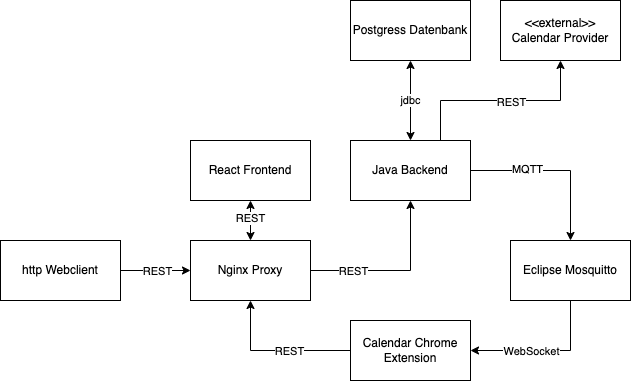
\includegraphics[width=0.85\textwidth]{../figures/implementation-claendar-companion-system.drawio.png}
      \caption{Systemübersicht zur Kalenderintegration in Yappi}
      \label{fig:implementation-calendar-companion-system}
    \end{figure}

    Die Abbildung~\ref{fig:implementation-calendar-companion-system} zeigt eine Systemübersicht der Kalenderintegration.

\subsubsection{Backend-Integration}

    Das Kalendermodul ist für die Verwaltung und Bereitstellung von Kalendereinträgen verantwortlich.
    Es unterstützt sowohl den Abruf von Einträgen über eine REST-API als auch eine proaktive Benachrichtigung von Clients in Echtzeit.
    Letzteres erfolgt über das Publish-Subscribe-Protokoll \textit{MQTT} (Message Queuing Telemetry Transport).
    Zudem werden externe iCalendar-Daten (ICS) der Nutzer automatisch synchronisiert.

\paragraph{Model-Klasse}
    Die zentrale Datenstruktur bildet die JPA-Entität \texttt{CalendarEvent.java} (\texttt{entities/}).
    Sie repräsentiert einen einzelnen Kalendereintrag mit Attributen wie \texttt{title}, \texttt{startDate}, \texttt{endDate}, \texttt{allDay} sowie der Zuordnung zu einem Nutzer (\texttt{userId}).
    Diese Klasse wird innerhalb des Backends zwischen Services und Controllern verwendet.

\paragraph{API-Endpunkte (\texttt{CalendarController})}
    Die Interaktion externer Clients mit dem Kalendermodul erfolgt über folgende REST-Endpunkte:
    \begin{itemize}
        \item \texttt{GET /api/calendar/\{userId\}}
            Ruft alle Kalendereinträge einer bestimmten Nutzer-ID ab.
            Der Controller delegiert die Anfrage an den \texttt{CalendarService}, der die Daten lädt und als JSON zurückgibt.
        \item \texttt{POST /api/calendar/sync}
            Stösst die Synchronisation manuell an, z.\,B. für sofortige Aktualisierungen oder Debugging.
            Nutzt dieselbe Logik wie die automatische Synchronisation durch den \texttt{CalendarEventScheduler}.
    \end{itemize}

\paragraph{Service-Schicht (\texttt{CalendarService})}
    Der \texttt{CalendarService} enthält die Geschäftslogik und entkoppelt Controller und geplante Aufgaben von der Datenverarbeitung.
    Er übernimmt:
    \begin{itemize}
        \item Abruf von Kalendereinträgen,
        \item Erstellung und Aktualisierung von Einträgen durch Abgleich mit externen Daten,
        \item Benachrichtigung über \texttt{MQTT} nach dem Ende von Terminen.
    \end{itemize}

\paragraph{Geplante Aufgaben (\texttt{CalendarEventScheduler})}
    Zwei periodische Jobs sorgen für Aktualität und Benachrichtigungen:
    \begin{enumerate}
        \item \textbf{Prüfung beendeter Events} (alle 60 Sekunden):
            Erkennt neu abgeschlossene Kalendereinträge und benachrichtigt betroffene Clients über \texttt{MQTT}.
        \item \textbf{Kalendersynchronisation} (alle 5 Minuten):
            Aktualisiert Kalendereinträge auf Basis externer ICS-Daten.
            Dabei werden neue Events erstellt, geänderte aktualisiert und nicht mehr vorhandene gelöscht.
            Änderungen lösen eine Update-Benachrichtigung an die Clients aus.
    \end{enumerate}

\paragraph{Echtzeit-Benachrichtigungen (\texttt{MqttService})}
    Nach Änderungen publiziert der \texttt{MqttService} Nachrichten auf themenspezifischen Topics (z.\,B. \texttt{deardev/teams/\{teamId\}/calendar}).
    Clients abonnieren diese Topics und können ihre UI unmittelbar aktualisieren, ohne Polling durchführen zu müssen.


\subsubsection{Datenbankerweiterung}

    Zur Speicherung der Kalendereinträge wurde die neue Tabelle \texttt{calendar\_events} eingeführt.
    Die Struktur wird durch die JPA-Entität \texttt{CalendarEvent.java} definiert.

\begin{table}[!htbp]
    \centering
    \begin{tabular}{|l|l|p{9cm}|}
        \hline
            \textbf{Spalte} & \textbf{Datentyp} & \textbf{Beschreibung} \\
        \hline
            \texttt{id} & INTEGER & Primärschlüssel des Eintrags \\
            \texttt{title} & VARCHAR & Titel des Kalenderevents (z.\,B. \glqq Sprint~1\grqq) \\
            \texttt{start\_date} & TIMESTAMP & Startdatum und -zeit \\
            \texttt{end\_date} & TIMESTAMP & Enddatum und -zeit \\
            \texttt{all\_day} & BOOLEAN & Kennzeichen für ganztägige Events \\
            \texttt{user\_id} & INTEGER & Fremdschlüssel zur Tabelle \texttt{users} \\
            \texttt{team\_id} & INTEGER & Fremdschlüssel zur Tabelle \texttt{teams} \\
        \hline
    \end{tabular}
    \caption{Schema der Tabelle \texttt{calendar\_events}}
    \label{tab:calendar_events_schema}
\end{table}

\paragraph{Backend-Komponenten}
    \begin{itemize}
        \item \textbf{Entität} (\texttt{CalendarEvent.java}): Datenmodell und Tabellenstruktur.
        \item \textbf{Repository} (\texttt{CalendarEventRepository.java}): CRUD-Operationen auf \texttt{calendar\_events}.
        \item \textbf{Service} (\texttt{CalendarService.java}): Geschäftslogik zum Erstellen, Abrufen und Löschen von Events.
        \item \textbf{Controller} (\texttt{CalendarController.java}): REST-Endpunkte zum Abrufen von Events pro Nutzer.
        \item \textbf{Scheduler} (\texttt{CalendarEventScheduler.java}): Zeitgesteuerte Erstellung und Aktualisierung der Events.
        \item \textbf{Factory} (\texttt{CalendarEventFactory.java}): Hilfsklasse zur einfachen Erstellung neuer Eventobjekte.
    \end{itemize}

\paragraph{Automatisierte Erstellung}
    Der \texttt{CalendarEventScheduler} generiert automatisch Einträge auf Basis aktiver Sprints:
    \begin{enumerate}
        \item Abruf aller aktiven Sprints für jedes Team,
        \item Prüfung, ob für jedes Teammitglied bereits ein Event existiert,
        \item Erstellung neuer Events mittels \texttt{CalendarEventFactory}, falls erforderlich,
        \item Speicherung der Events über das \texttt{CalendarEventRepository}.
    \end{enumerate}

\subsubsection{Kommunikationsbroker}
    Für die Echtzeitübertragung von Benachrichtigungen an Clients wird der Open-Source-MQTT-Broker \textbf{Eclipse Mosquitto} eingesetzt.
    \textit{MQTT} (Message Queuing Telemetry Transport) ist ein leichtgewichtiges Publish-Subscribe-Protokoll, das sich besonders für Anwendungen mit geringer Latenz und hohem Aktualisierungsbedarf eignet.

\paragraph{Zweck}
    Der Kommunikationsbroker ermöglicht die sofortige Benachrichtigung von Companion-Anwendungen, insbesondere der Google-Chrome-Erweiterung des Calendar Companions.
    Damit entfällt die Notwendigkeit von Polling-Anfragen an das Backend, was die Netzwerklast reduziert und eine reaktive Benutzeroberfläche ermöglicht.

\paragraph{Kommunikationsfluss}
    \begin{enumerate}
        \item Das Backend erkennt eine relevante Änderung, z.\,B. das Ende eines Meetings oder die Erstellung eines neuen Kalendereintrags.
        \item Der \texttt{MqttService} des Backends verbindet sich mit dem Mosquitto-Broker und publiziert die Nachricht auf einem benutzerspezifischen Topic:
            \texttt{calendar/event/\{user-api-key\}}.
        \item Die Chrome-Erweiterung des Calendar Companions ist als MQTT-Client auf diesem Topic angemeldet (\textit{subscribed}).
        \item Beim Empfang einer Nachricht aktualisiert der Client die lokale Ansicht und kann bei Bedarf Folgeaktionen anstossen (z.\,B. Anzeige eines Feedback-Dialogs).
    \end{enumerate}

\paragraph{Nachrichtenformat}
    Die vom Backend publizierten Benachrichtigungen werden als JSON-Objekte gesendet.
    Eine typische Nachricht enthält die folgenden Felder:

    \begin{verbatim}
        {
            "eventId": 3002,
            "userId": 1,
            "title": "Meeting IP5 - Standup",
            "startDate": "2025-08-09T15:00",
            "endDate": "2025-08-09T15:15",
            "location": "",
            "questionBlockId": 1,
            "teams": [
                {
                    "id": 1,
                    "name": "Test Team 1"
                },
                {
                    "id": 3,
                    "name": "Test Team 2"
                }
            ]
        }
    \end{verbatim}

\paragraph{Vorteile}
    \begin{itemize}
        \item Sofortige Zustellung ohne Polling.
        \item Geringe Netzwerklast durch Publish-Subscribe-Architektur.
        \item Einfaches Routing über benutzerspezifische Topics.
        \item Erweiterbar für weitere Eventtypen oder Companion-Anwendungen.
    \end{itemize}


\subsubsection{Yappi Chrome Extension}
    Die Yappi Chrome Extension dient als Companion-Anwendung zur Erfassung von Zufriedenheits-Feedback und Benachrichtigen
    über das beenden von Kalendereinträgen direkt im Webbrowser.
    Sie ist als ereignisgesteuerte Anwendung konzipiert und unterstützt sowohl synchrone Datenabfragen als auch
    asynchrone Echtzeitbenachrichtigungen.

    Die Extension ermöglicht es, Umfragen und Benachrichtigungen ohne den Umweg über die Yappi-Webplattform zu verarbeiten.
    Dadurch werden Feedbackprozesse in den Arbeits Flow des Nutzers verlagert und Befragungsmüdigkeit reduziert.

\paragraph{Architektur}
    Die Anwendung besteht aus zwei Hauptkomponenten:
    \begin{enumerate}
      \item \textbf{Persistenter Background-Prozess}
            Läuft dauerhaft im Hintergrund und ist für die Kommunikation mit externen Diensten, die Verwaltung des Zustands
            und das proaktive Benachrichtigen des Nutzers zuständig.
      \item \textbf{Temporäre Popup-Benutzeroberfläche (UI)}
            Wird nur bei aktiver Benutzerinteraktion geladen und dient der Darstellung von Inhalten sowie der Erfassung von Feedback.
    \end{enumerate}


\paragraph{Kommunikationskanäle}
    Die Verbindung zum Yappi-Backend erfolgt über zwei Kanäle:
    \begin{itemize}
      \item \textbf{REST-API} Für synchronen Abruf von Daten (z.\,B. Umfragen) und Übermittlung von Antworten.
      \item \textbf{MQTT-Broker} Für asynchrone Benachrichtigungen in Echtzeit, z.\,B. über neu verfügbare Umfragen.
    \end{itemize}
    Die interne Kommunikation zwischen Background-Prozess und Popup-UI nutzt die Browser-API \texttt{chrome.storage}.

\paragraph{Komponenten im Detail}
    \subparagraph{Background-Prozess (\texttt{background/background.js})}
        \begin{itemize}
          \item Aufbau und Aufrechterhaltung einer MQTT-Verbindung (über \texttt{lib/mqtt.js}) zu einem Broker via WebSocket.
          \item Abonnieren benutzerspezifischer Topics zur Echtzeitbenachrichtigung.
          \item Verarbeitung eingehender Nachrichten und Erzeugung nativer Desktop-Benachrichtigungen (\texttt{chrome.notifications}).
          \item Persistente Speicherung der letzten zehn Ereignisse in \texttt{chrome.storage.local} nach FIFO-Prinzip.
        \end{itemize}


    \subparagraph{Popup-Benutzeroberfläche (\texttt{popup/home.html})}
        \begin{itemize}
          \item Dynamischer Umfrage-Builder (\texttt{popup/survey/builder.js}):
                Ruft aktuelle Umfragen über die REST-API ab, generiert DOM-Elemente aus Vorlagen (\texttt{popup/questionblock.html},
                \texttt{popup/questionblock.js}) und integriert diese in die Ansicht.
          \item Feedback-Übermittlung (\texttt{popup/popup.js}):
                Sammelt Antworten, strukturiert sie als JSON und sendet sie per POST-Request an die REST-API.
          \item Verlaufsansicht (\texttt{popup/history.html}, \texttt{popup/history.js}):
                Liest die letzten zehn gespeicherten Ereignisse aus und stellt sie in einer separaten Ansicht dar.
        \end{itemize}

\paragraph{Externe Abhängigkeiten}
    \begin{itemize}
      \item \textbf{Yappi-Backend} Bereitstellung der REST-API und MQTT-Broker.
      \item \textbf{MQTT.js} (\texttt{lib/mqtt.js}) JavaScript-Clientbibliothek für MQTT-Kommunikation.
    \end{itemize}

\subsubsection{Dynamische Umfragen}
    Die dynamischen Umfragen in Yappi basieren auf flexibel konfigurierbaren Fragenblöcken, die als JSON-Objekte in der Datenbank gespeichert werden.
    Diese Struktur ermöglicht es, Umfragen anzupassen oder zu erweitern, ohne Änderungen am Anwendungscode vorzunehmen.

\paragraph{Datenbank}
    Die Tabelle \texttt{questionblocks} speichert die Konfiguration einzelner Fragenblöcke.

    \begin{table}[!htbp]
        \centering
        \begin{tabular}{|l|l|p{9cm}|}
            \hline
                \textbf{Spalte} & \textbf{Datentyp} & \textbf{Beschreibung} \\
            \hline
                \texttt{id} & SERIAL & Eindeutiger, automatisch inkrementierender Primärschlüssel \\
                \texttt{configuration} & JSONB & Vollständige Konfiguration des Fragenblocks als JSON-Objekt.
                Ermöglicht flexible Strukturierung und effiziente Abfragen \\
            \hline
        \end{tabular}
        \caption{Schema der Tabelle \texttt{questionblocks}}
        \label{tab:questionblocks_schema}
    \end{table}

    \noindent
    \textbf{Anmerkung:} Der Datentyp \texttt{JSONB} (Binary JSON) erlaubt eine performante Speicherung und gezielte Abfragen innerhalb der JSON-Daten.

\paragraph{Backend-Komponenten}
    \begin{itemize}
        \item \textbf{Entität} (\texttt{QuestionBlock.java}) — Abbildung der Tabelle \texttt{questionblocks} als JPA-Entität.
            Attribute: \texttt{id} (INTEGER) und \texttt{configuration} (\texttt{JsonNode}).
        \item \textbf{Repository} (\texttt{QuestionBlockRepository.java}) — CRUD-Operationen auf der Tabelle.
        \item \textbf{Service} (\texttt{QuestionBlockService.java}) — Geschäftslogik für den Zugriff und die Validierung von Fragenblöcken.
        \item \textbf{Controller} (\texttt{QuestionBlockController.java}) — Bereitstellung der API-Endpunkte.
    \end{itemize}

\paragraph{API-Endpunkte}
    \begin{itemize}
        \item \texttt{GET /companion/questionblocks/\{id\}}
            Ruft den Fragenblock mit der angegebenen ID ab.
            \textbf{Antworten:} \texttt{200 OK} mit JSON-Objekt oder \texttt{404 Not Found}, falls nicht vorhanden.
    \end{itemize}

\paragraph{Darstellung in der Companion-App}
    Die Chrome Extension ruft den entsprechenden Fragenblock per REST-API ab.
    Das Skript \texttt{popup/survey/builder.js} parst die JSON-Daten und erstellt für jede Frage die passenden HTML-Elemente
    basierend auf den Templates (\texttt{popup/questionblock.html}) und der Logik in \texttt{popup/questionblock.js}.
    Unterstützt werden Fragetypen wie:
    \begin{itemize}
        \item Likert-Skalen
        \item Single-Choice
        \item Multiple-Choice
        \item Freitext
    \end{itemize}

\paragraph{Beispiel einer Umfragekonfiguration}
    \begin{verbatim}
        {
        "id": "1000",
        "title": "Basic Meeting Feedback",
        "description": "This is am Meeting feedback survey.",
        "sections": [
        {
            "id": "q1",
            "type": "likert",
            "title": "1. Clarity of Goals & Relevance",
            "prompt": "The goals of the meeting were clearly defined.",
            "required": true,
            "min": 1,
            "label_min": "strongly disagree",
            "max": 5,
            "label_max": "strongly agree",
            "step": 1,
            "default": 3
        },
        {
            "id": "q2",
            "type": "single-choice",
            "title": "2. Meeting Length",
            "prompt": "How would you rate the length of the meeting?",
            "required": true,
            "options": [
                { "value": "too-short", "label": "Too short" },
                { "value": "just-right", "label": "Just right" },
                { "value": "too-long", "label": "Too long" }
            ],
            "default": "just-right"
        },
        {
        "id": "q3",
        "type": "multiple-choice",
        "title": "3. Meeting Highlights",
        "prompt": "Which aspects of the meeting did you find valuable? (Select all that apply)",
        "required": false,
        "options": [
            { "value": "clear-agenda", "label": "Clear agenda" },
            { "value": "useful-content", "label": "Useful content" },
            { "value": "good-discussion", "label": "Good discussion" },
            { "value": "action-items", "label": "Clear action items" }
        ],
        "default": ["clear-agenda", "good-discussion"]
        },
        {
            "id": "q5",
            "type": "free-text",
            "title": "4. Additional Comments",
            "prompt": "Please share any additional feedback or suggestions.",
            "required": false,
            "placeholder": "Type your feedback here...",
            "maxLength": 500
        }
        ]
        }
    \end{verbatim}

\paragraph{Vorteile}
    \begin{itemize}
        \item Anpassung und Erweiterung von Umfragen ohne Codeänderungen.
        \item Unterstützung verschiedener Fragetypen und Layouts.
        \item Zentrale Verwaltung und Wiederverwendung von Fragenblöcken.
    \end{itemize}


\todo{Sequenzdiagramm}
\todo{Front End Anpassung}

\subsection{Health Companion}

\todo{Health Kit API}
\todo{Kommunikation}
\todo{Benutzeroberfläche}
\todo{Datenbankerweiterung}

\section{Deployment}
\xeno{}
\todo{UML Deployment Diagramm}

\chapter{Evaluation}
\xeno{}
\todo{Hackathon}
\todo{kleine evaluation vor projektende}
\section{Beantwortung der Fragestellung}

\chapter{Diskussion}

\printbibliography

\end{document}
